\section{Renewable Resources\label{sec-intro-renewable}}
The results of this work are based on the utilization of renewable resources, which is introduced in the first subsection. One such renewable resource is \lcbm{}. It is used a basis for \lch{}, a man-made product from \lcbm{}. As \lch{} is the starting material used in this work, commonly encountered issues stemming from the production method and remedies for them are presented herein.

\subsection{Definition: What Makes a Resource Renewable?\label{subsec-intro-renewable-def}}
The definition given by \textcite{Weiss1962} is limited to \enquote{[...] the total range of living organisms providing man with food, fibers, drugs, etc., for his needs [...]}. Probably, the most elaborate definition of what constitutes renewable resources is given by \textcite{Armstrong1999} and does not include life forms other than plants:
\begin{quote}
The term \enquote{renewable} is generally applied to those energy resources and technologies whose common characteristic is that they are non-depletable or naturally replenishable.

Renewable resources include solar energy, wind, falling water, the heat of the earth (geothermal), plant materials (biomass), waves, ocean currents, temperature differences in the oceans and the energy of the tides. Renewable energy technologies produce power, heat or mechanical energy by converting those resources either to electricity or to motive power. [...]
\end{quote}

Thus, one property of renewable resources is a non-depletable supply. This must not be mistaken for an infinite supply and one should be wary not to overuse such resources and its renewing character must be managed properly \cite{Moxnes1998}.

\nomenclature[latabbr_IUCN]{IUCN}{International Union for Conservation of Nature and Natural Resources}
\begin{figure}
	\begin{center}
		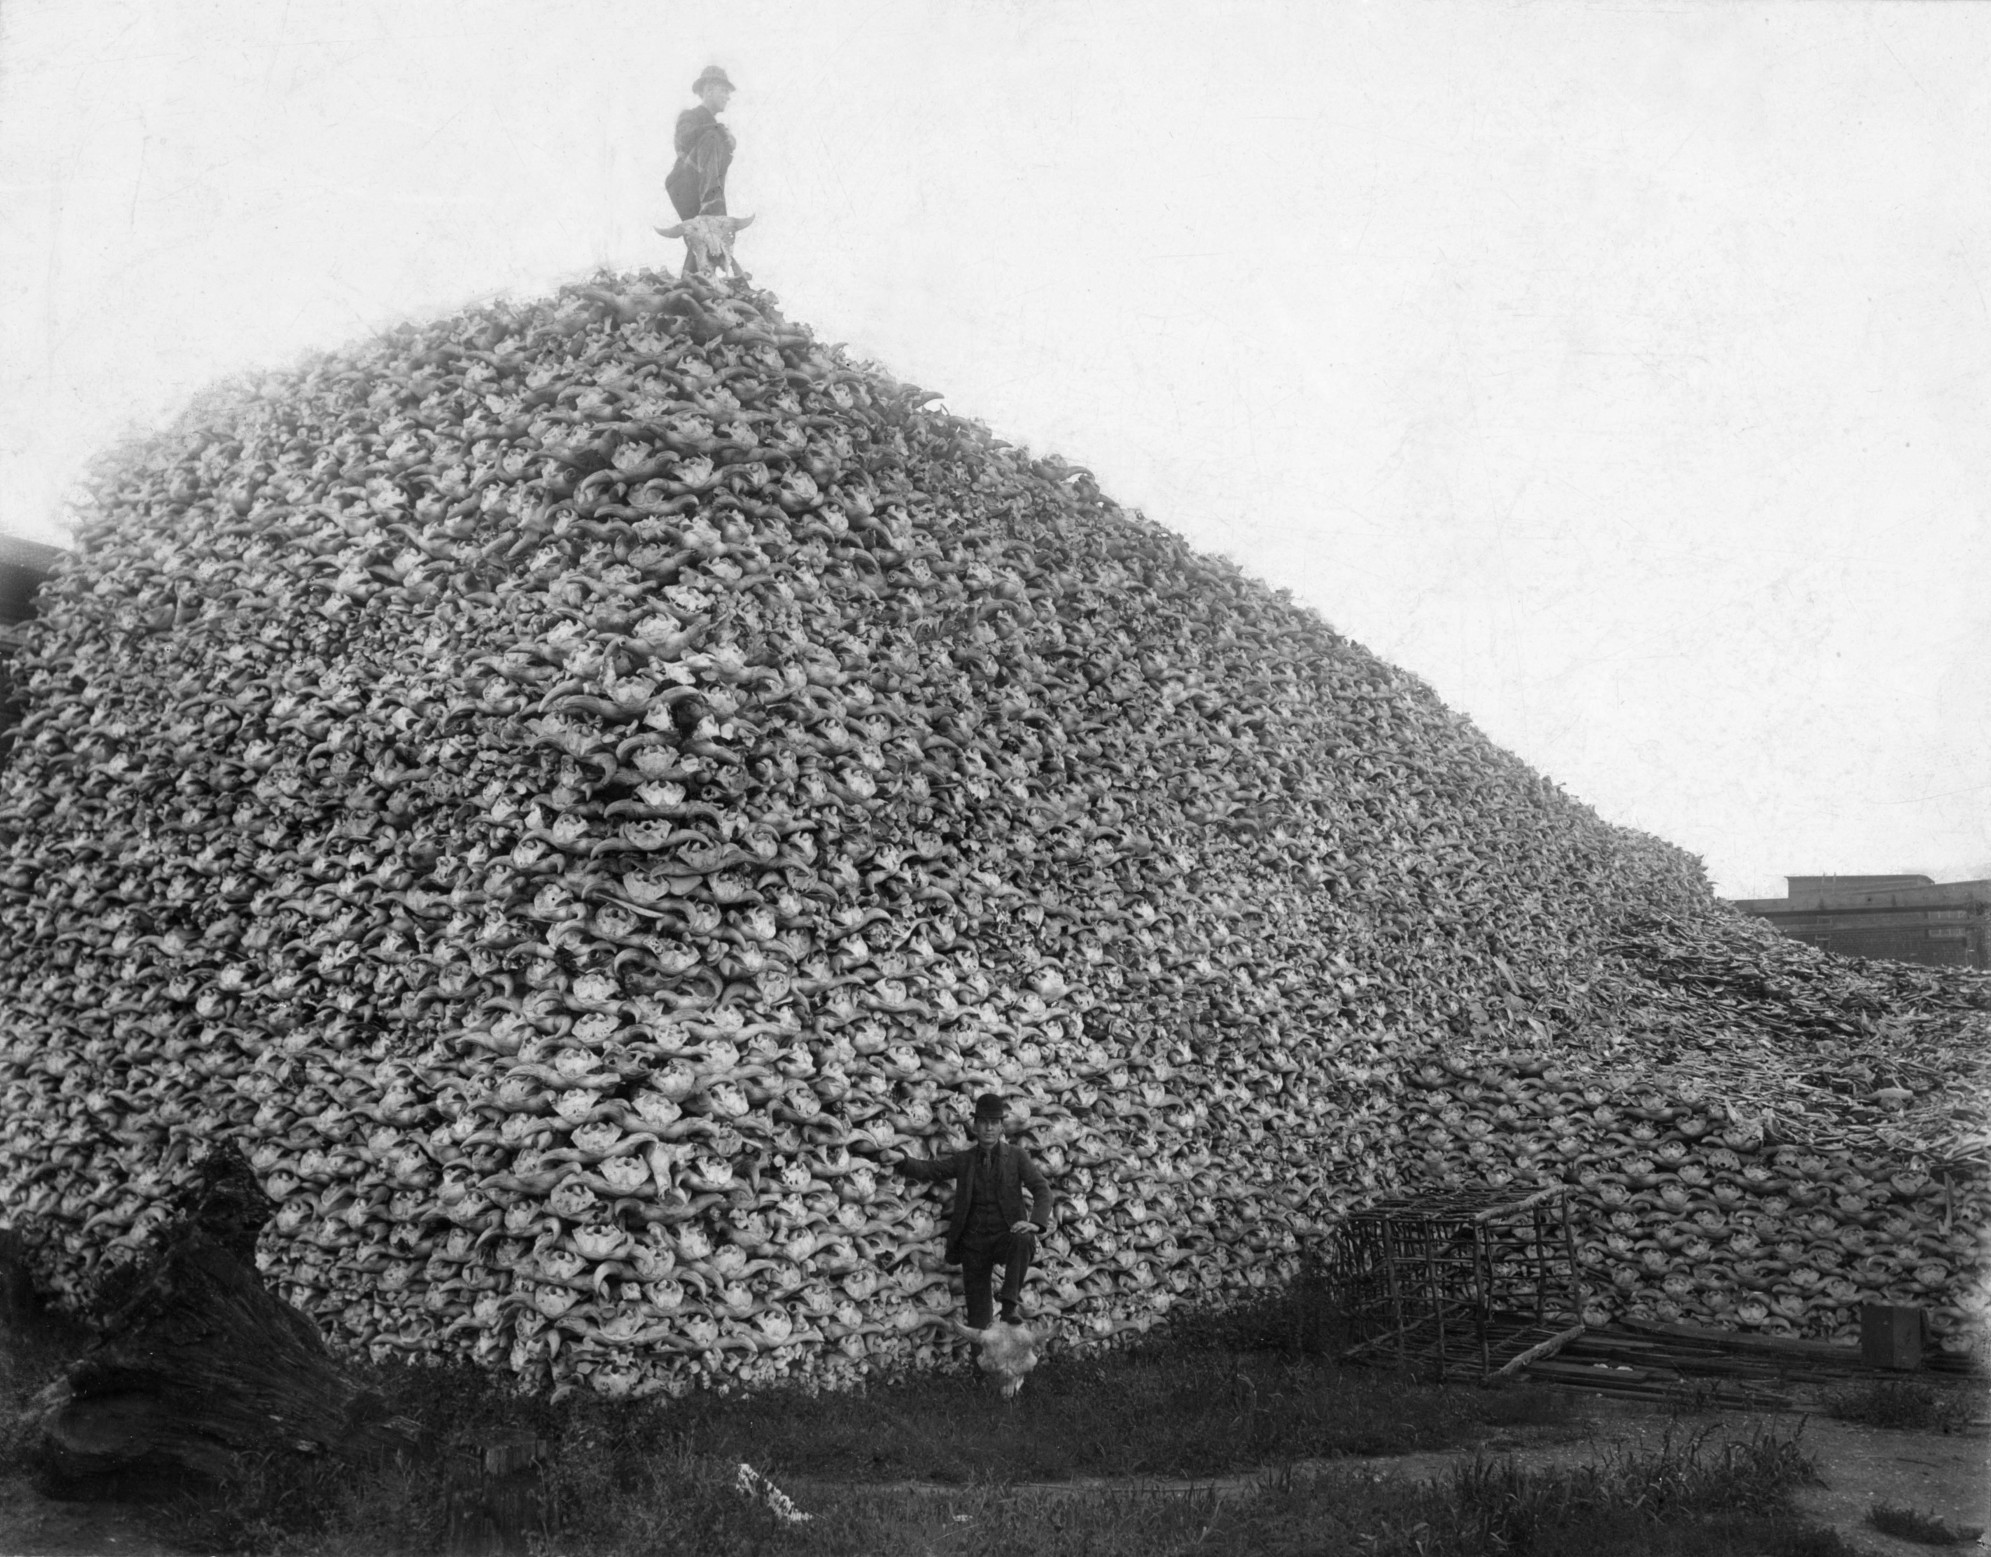
\includegraphics[width=\textwidth]{fig/Bison_skull_pile_grey_stretched_small.jpg}
		\caption[Overuse of Renewable Resources: A Pile of Bison Skulls]{Photograph from the mid-1870s of a pile of American bison skulls waiting to be ground for fertilizer \cite{Anonymous1870}. At the outset of the 19th century, between \num{30} million and \num{75} million bisons roamed North America. After a century of reckless hunting and exploitation of this renewable resource, less than \num{300} individuals remained \cite{USFWS1997}. Nowadays, the American buffalo is listed as \enquote{Near Threatened} on the IUCN Red List of Threatened Species \cite{IUCNRedList20154}.\label{fig-intro-renewable-overuse}}
	\end{center}
\end{figure}

An infamous example of mismanagement of a renewable resource is the hunting of the American bison in North America in the 19th century. It is estimated that around \num{30} million to \num{75} million bisons roamed North America in 1800. After just a hundred years, the number was reduced to less than \num{300} due to reckless hunting and exploitation of this renewable animal resource \cite{USFWS1997}. \Vref{fig-intro-renewable-overuse} depicts a pile of bison skulls from the mid-1870s. The number of skulls is estimated to be on the order of \num{100000} and serves as a graphic example for the shortsighted mindset present at that time. The aftermath is still visible even today, more than a century later: the species is listed as \enquote{Near Threatened} on the IUCN Red List of Threatened Species \cite{IUCNRedList20154}.

Therefore, when exploiting renewable resources, man must always keep in mind that the rates of renewal and consumption must be sustainable on a long term. Not only commercial considerations, but also the responsibility for the future generations mandate efficient use of renewable resources.

\subsection{\LCBM{}: The Most Abundant Renewable Carbon Resource\label{subsec-intro-renewable-lcbm}}
\begin{figure}
	\subfloat[\textit{p}-Coumaryl alcohol]{
			\label{fig-intro-pcoum}%
			\includegraphics[width=0.3\textwidth]{fig/Molecule_p-coumaryl_alcohol_600dpi.png}
	}
	\hfill
	\subfloat[Coniferyl alcohol]{
			\label{fig-intro-coni}%
			\includegraphics[width=0.3\textwidth]{fig/Molecule_coniferyl_alcohol_600dpi.png}
	}
	\hfill
	\subfloat[Sinapyl alcohol]{
			\label{fig-intro-sina}%
			\includegraphics[width=0.3\textwidth]{fig/Molecule_sinapyl_alcohol_600dpi.png}
	}

	\subfloat[Phenol]{
			\label{fig-intro-phenol}%
			\includegraphics[width=0.3\textwidth]{fig/Molecule_phenol_600dpi.png}
	}
	\hfill
	\subfloat[Guaiacol]{
			\label{fig-intro-guaiacol}%
			\includegraphics[width=0.3\textwidth]{fig/Molecule_guaiacol_600dpi.png}
	}
	\hfill
	\subfloat[Syringol]{
			\label{fig-intro-syringol}%
			\includegraphics[width=0.3\textwidth]{fig/Molecule_syringol_600dpi.png}
	}
	\caption[Phenylpropanoid Precursors and Eponymous Molecules of Lignin]{Phenylpropanoid precursors and eponymous molecules of lignin. \subref*{fig-intro-pcoum}, \subref*{fig-intro-coni} and \subref*{fig-intro-sina}: Phenylpropanoid precursors of lignin \cite{Adler1977}. \subref*{fig-intro-phenol}, \subref*{fig-intro-guaiacol} and \subref*{fig-intro-syringol}: Structures of the eponymous molecules for phenolics (\subref*{fig-intro-phenol}), guaiacyl lignins (\subref*{fig-intro-guaiacol}) and syringyl lignins (\subref*{fig-intro-syringol}). The structural difference between guaiacyl lignins and guaiacyl-syringyl lignins is an additional methoxy group in syringyl lignins, which can also be seen in the structures of the building blocks of lignin, coniferyl alcohol (\subref*{fig-intro-coni}) and sinapyl alcohol (\subref*{fig-intro-sina}) \cite{Saka2001}.\label{fig-intro-renewable-lcbm-lignin-precursors}}
\end{figure}

The production of lignocellulose is estimated to exceed \SI{1E12}{\tonne\per\year} and is the major renewable carbon source on planet Earth \cite{Hon1992, Mohanty2000}. In contrast, the world crude oil production in 2014 was \SI{4.24E9}{\tonne} \cite{DERA2015}, less than one percent of the annual lignocellulose production. However, as outlined above, renewable resources must be managed wisely and as of now fossil fuels are clearly dominating the fuel market.

The main components of \lcbm{} are the two eponymous ones lignin and cellulose and a third one called hemicellulose. All three are densely packed: cellulose fibrils are encased by hemicellulose which is chemically bound to lignin \cite{Palmqvist2000b}. Examples of \lcbm{} are wood and grass, but also wastes and residues from forestry, agriculture or municipalities.

In wood, the three aforementioned components are the main constituents as well. Wood can be classified as \enquote{softwood} or \enquote{hardwood}. The differences between softwood and hardwood lie within the relative proportions of lignin, cellulose and hemicellulose and structural details \cite{Palmqvist2000b}. Examples of softwoods are pine and spruce and examples of hardwoods are aspen, oak and willow \cite{Saka2001}. Compositions of different \lcbm{}es were reported by \textcite{Sun2002}.

The word \enquote{lignin} derives from the Latin word \textit{lignum} meaning \enquote{wood}. Lignin is a polymer synthesized from phenylpropanoid precursors \cite{Adler1977, Palmqvist2000b}. Examples for these precursors are given in \vref{fig-intro-renewable-lcbm-lignin-precursors}. Based on the precursors, two lignin classes can be distinguished: guaiacyl lignins and guaiacyl-syringyl lignins. The structural difference of guaiacyl lignins and guaiacyl-syringyl lignins is an additional methoxy group at position 5 in syringyl lignins. While softwoods contain guaiacyl lignins, hardwoods contain guaiacyl-syringyl lignins. Overall, softwoods contain more lignin than hardwoods \cite{Saka2001}.

Cellulose consists of unbranched linear \glc{} monomers exclusively. The single \glc{} units are β-1,4-linked and the resulting polymer can be a highly crystalline or an amorphous material \cite{Fan1982}. Crystalline cellulose is more difficult to degrade microbially than amorphous cellulose \cite{Beguin1994}. Nonetheless, microbial degradation of crystalline cellulose is possible \cite{Klyosov1986, Beeson2015}.

On the other hand, hemicelluloses are irregular branched polysaccharides which consist of pentoses, hexoses and uronic acids such as \ara{}, \xyl{}, \gal{}, \glc{}, \man{}, \glcua{} and \galua{} \cite{Saka2001}. The hemicellulose of hardwoods is more highly acetylated than in softwoods and contains a higher proportion of \xyl{}, while softwood hemicelluloses contain higher proportions of \glc{} and \man{} than hardwood hemicellulose \cite{Fengel1989}.

\subsection{\LCH{}: A Man-Made Degradation Product\label{subsec-intro-renewable-lch}}
\begin{figure}
	\subfloat[\Fora{}]{
			\label{fig-intro-form}%
			\includegraphics[width=0.0977\textwidth]{fig/Molecule_formic_acid_600dpi.png}
	}
	\hfill
	\subfloat[\Acet{}]{
			\label{fig-intro-acet}%
			\includegraphics[width=0.0825\textwidth]{fig/Molecule_acetic_acid_600dpi.png}
	}
	\hfill
	\subfloat[\Laev{}]{
			\label{fig-intro-laev}%
			\includegraphics[width=0.217\textwidth]{fig/Molecule_laevulinic_acid_600dpi.png}
	}
	\hfill
	\subfloat[\FUR{}]{
			\label{fig-intro-fur}%
			\includegraphics[width=0.121\textwidth]{fig/Molecule_furfural_600dpi.png}
	}
	\hfill
	\subfloat[\HMF{}]{
			\label{fig-intro-hmf}%
			\includegraphics[width=0.198\textwidth]{fig/Molecule_hydroxymethylfurfural_600dpi.png}
	}

	\subfloat[Syringaldehyde]{
			\label{fig-intro-syr}%
			\includegraphics[width=0.234\textwidth]{fig/Molecule_syringaldehyde_600dpi.png}
	}
	\hfill
	\subfloat[\VAN{}]{
			\label{fig-intro-van}%
			\includegraphics[width=0.156\textwidth]{fig/Molecule_vanillin_600dpi.png}
	}
	\hfill
	\subfloat[\Ga{}]{
			\label{fig-intro-ga}%
			\includegraphics[width=0.170\textwidth]{fig/Molecule_gallic_acid_600dpi.png}
	}
	\hfill
	\subfloat[\pHba{}]{
			\label{fig-intro-phba}%
			\includegraphics[width=0.170\textwidth]{fig/Molecule_4-hydroxybenzoic_acid_600dpi.png}
	}
	\caption[Selected Inhibitors From Lignocellulose Hydrolysis]{
Selected inhibitors of microbial growth released and/or formed during \lch{} production.
\Fora{} (\subref*{fig-intro-form}) is a degradation product of \fur{} (\subref*{fig-intro-fur}) \cite{Grote1875, Dunlop1948} and \hmf{} (\subref*{fig-intro-hmf}).
\Acet{} (\subref*{fig-intro-acet}) is freed from acetylated hemicellulose.
\Laev{} (\subref*{fig-intro-laev}) is a degradation product of \hmf{} (\subref*{fig-intro-hmf}) \cite{Horvat1985}.
\FUR{} (\subref*{fig-intro-fur}) is degradation product of C5 sugars, e.g. \xyl{} \cite{Dunlop1948}.
\HMF{} (\subref*{fig-intro-hmf}) is a degradation product of C6 sugars, e.g. \glc{} \cite{Heimlich1960, Feather1970, Taylor1972, Fukuchi1977}, \man{} or \gal{}.
Phenolic compounds such as \syr{} (\subref*{fig-intro-syr}), \van{} (\subref*{fig-intro-van}), \ga{} (\subref*{fig-intro-ga}) or \phba{} (\subref*{fig-intro-phba}) are degradation products of lignin \cite{Bardet1985, Lapierre1983, Sears1971} or carbohydrates \cite{Popoff1976, Suortti1983}.\label{fig-intro-renewable-lch-inhibitors}}
\end{figure}

With its plethora of sugars, especially \glc{} and \xyl{}, \lcbm{} is a good candidate for microbial utilization. In order to make these resources available for fermentation processes, the recalcitrant structures of \lcbm{} need to be broken and the sugar monomers freed. The resulting product of such a process is called \lch{}. Different treatments exist to convert \lcbm{} into \lch{} and gain the highest amount of sugars. Unfortunately, dilute acid hydrolysis, a commonly employed treatment, is accompanied by the formation of inhibitors of microbial growth \cite{Sun2002, Klinke2004}. For this work, the inhibitors formed during preparation of such dilute acid \lch{}s are the most important ones and are covered in some detail below. Neither the chemical explanations for inhibitor formation nor inhibition mechanisms or general detoxification strategies are covered. Advantages and disadvantages of the different (pre-)treatment methods are covered by \textcite{Brodeur2011}, while inhibitor formation, inhibition mechanisms and general detoxification strategies are described in detail in the two reviews by \textcite{Palmqvist2000a, Palmqvist2000b}.

\subsubsection{Inhibitors of Microbial Growth}
\nomenclature[chem_C5 sugar]{C5 sugar}{sugar with five carbon atoms}
\nomenclature[chem_C6 sugar]{C6 sugar}{sugar with six carbon atoms}
A selection of different inhibitors formed during dilute acid hydrolysis of \lcbm{} is presented in \vref{fig-intro-renewable-lch-inhibitors}. Subfigures \subref*{fig-intro-form}, \subref*{fig-intro-acet} and \subref*{fig-intro-laev} show the structures of formic, acetic and \laev{}, respectively. While \fora{} is a degradation product of \fur{} \cite{Grote1875, Dunlop1948} and \hmf{}, \laev{} is a degradation product of only \hmf{} \cite{Horvat1985}. \Acet{} is freed from the acetylated hemicellulose. Subfigures \subref*{fig-intro-fur} and \subref*{fig-intro-hmf} depict the structures of the furan derivatives \fur{} and \hmf{}, respectively. \FUR{} is a degradation product of C5 sugars \cite{Dunlop1948} and \hmf{} is a degradation product of C6 sugars \cite{Heimlich1960, Feather1970, Taylor1972, Fukuchi1977}. The phenolic compounds \syr{}, \van{}, \ga{} and \phba{} are depicted in subfigures \subref*{fig-intro-syr}, \subref*{fig-intro-van}, \subref*{fig-intro-ga} and \subref*{fig-intro-phba}, respectively. They are degradation products of lignin \cite{Bardet1985, Lapierre1983, Sears1971} or carbohydrates \cite{Popoff1976, Suortti1983}.

\subsubsection{Microbial Detoxification}
The use of \lch{} as a substrate for microorganisms is hampered by the presence of inhibitors. It is likely that the negative effect on microbial growth increases from aliphatic organic acids to furan derivatives to phenolics \cite{Larsson1999, Palmqvist2000a}. The inhibitory effect of mixtures of different types of inhibitors increases in a synergistic manner \cite{Palmqvist1999}.

\nomenclature[chem_CoA]{CoA}{coenzyme A}
Since most of the inhibitors occur naturally as well, it is no surprise that microorganisms have evolved mechanisms to detoxify these substances. Accounts of lignin degradation were shown not only for fungi \cite{Jonsson1998} but also for bacteria \cite{Reiter2013, Kosa2013}. Three enzymes from \mo{Sphingobium}~sp.~SYK6 were shown \enquote{to release lignin monomers from complex lignin structures coming from differently prepared real lignin substrates} \cite{Reiter2013}. Furan derivatives are detoxified by bacteria as well \cite{Brune1983, Boopathy1993, Koopman2010, Lopez2004a, Wierckx2011}. \HMF{} can be converted to a furan dicarboxylic acid and then to furoic acid, which uses the \fur{} degradation pathway \cite{Koopman2010}. In this pathway, \fur{} is first oxidized to furoic acid, bound to coenzyme A as 2-furoyl-CoA and converted to 5-hydroxy-2-furoyl-CoA. Following these steps, 2-oxo-glutaroyl-CoA is formed via keto-enol tautomerization and hydrolysis, which then enters the citric acid cycle as 2-oxo-glutaric acid \cite{Koopman2010}. The microbial utilization of \fora{} \cite{Stickland1929, Quayle1972, Friedrich1979} and \acet{} \cite{Herlihy1987, Wright1966} is well-established and almost trivial. \Laev{}, on the other hand, does not have a known natural source. Thus, microbial utilization of \laev{} cannot be taken for granted and the very limited amount of literature on microbial \laev{} utilization seems to emphasize this \cite{Sasaki1990, Jang1996, Steinbuechel1997, Keenan2004}. While all these publications describe the utilization of \laev{}, the biochemical background remains in the dark.

